\documentclass[sigconf,nonacm]{acmart}

\usepackage{amsmath}
\usepackage{amssymb}
\usepackage{amsthm}
\usepackage{algorithm}
\usepackage{algpseudocode}
\usepackage{booktabs}
\usepackage{graphicx}
\usepackage{xcolor}
\usepackage[inline]{enumitem}

\settopmatter{printacmref=false}
\renewcommand\footnotetextcopyrightpermission[1]{}
\pagestyle{plain}

\setcopyright{none}
\acmConference[]{}{}{}
\acmYear{2026}
\copyrightyear{2026}
\acmISBN{}
\acmDOI{}

\begin{document}

\title{The Traveling Flyerperson: A Concrete Exploration of Community, Computing, and Statistics in Cambridge, MA}

\author{Cambridge Developers}
\affiliation{
  \country{USA}
  \city{Cambridge}
  \state{MA}
}
% \email{contact@cambridge-dev.org}

\renewcommand{\shortauthors}{Cambridge Developers}

\begin{abstract}
We present \emph{The Traveling Flyerperson}, a project that begins with a mundane civic question---where should a small software collective place paper flyers in Cambridge, Massachusetts---and treats it as a substrate for serious work in algorithms, statistics, and community-scale computing. The deployed web application solves a Traveling Salesman Problem (TSP) over curated Cambridge locations using Nearest Neighbor, 2-Opt, and Brute Force solvers, exposes algorithm execution as a step-by-step debuggable visualization, and integrates OpenStreetMap-derived covariates (traffic signals, bulletin boards, transit) alongside an EXIF-grounded evidence registry of placed flyers. We then formalize the placement problem as a \emph{predictive estimation problem}: given a candidate location $L$, what is the expected conversion value of a flyer over its lifetime? We develop a unified framework that combines (i) interval-censored survival analysis via the Turnbull non-parametric maximum likelihood estimator (NPMLE) and Weibull accelerated failure time models for flyer lifespan, (ii) inhomogeneous Poisson point processes with non-stationary thinning to model legal and institutional removal dynamics, (iii) Gaussian-process Multi-Armed Bandits (GP-UCB, contextual GP-UCB, and HyperPrior Thompson Sampling) for sequential allocation, and (iv) a three-level Bayesian hierarchical model that fuses these components into a posterior conversion utility heatmap. The result is a small, defensible, end-to-end pipeline---from photograph to point process---that turns a community task into a tractable, technically rigorous research artifact.
\end{abstract}

\keywords{Traveling Salesman Problem, Bayesian hierarchical models, survival analysis, spatial point processes, multi-armed bandits, civic computing, Cambridge MA}

\maketitle

\section{Introduction}
\label{sec:intro}

Flyering is the most analog form of marketing that still routinely works. A volunteer prints a small stack of letter-sized posters, walks or bikes a circuit through a neighborhood, and tacks them onto bulletin boards inside cafes, laundromats, and libraries. The cost is a few dollars of toner and a few hours of pavement; the payoff is intentionally local. In Cambridge, Massachusetts---a city of dense pedestrian corridors, two large research universities, and a strong tradition of community boards---this practice remains a viable channel for small organizations to reach geographically and demographically targeted audiences \cite{cambridge-redditA, cambridge-redditB}.

The civic question we take seriously in this paper is short: \emph{where should we place these flyers, and how do we know?} A naive answer is to walk a route that visits a handful of well-known boards. A slightly less naive answer is to compute an optimal route through those boards. A serious answer is to recognize that route optimization is downstream of a more interesting estimation problem: each candidate location has a latent expected value that depends on how long a flyer is likely to survive there, how much foot traffic actually engages with it, and how legal and institutional regimes thin the population of postings over time \cite{mit-policy, duke-ordinances}.

This paper reports on a project---\emph{The Traveling Flyerperson}---that pursues this answer end to end. The deployed application (Section~\ref{sec:app}) is a SvelteKit static site hosted at \texttt{letters-cambridge.web.app/stories/flyering/}, which solves a TSP over curated Cambridge locations, exposes the underlying algorithms as a debuggable visualization, integrates OpenStreetMap covariate layers, and registers physical evidence of placement via EXIF GPS metadata. The mathematical framework (Sections~\ref{sec:survival}--\ref{sec:bhm}) treats the same problem as a Bayesian hierarchical estimation task. Section~\ref{sec:synthesis} draws operational conclusions, and Section~\ref{sec:discussion} reflects on what this project is really for: a small, public exercise in community, computing, and statistics done together \cite{cambridge-dev-org}.

\paragraph{Contributions.}
We make four concrete contributions:
\begin{enumerate}
    \item A deployed, mobile-first, client-side TSP visualization with three solvers, theming, evidence registry, and OpenStreetMap layer integration.
    \item A unified mathematical framework for flyer placement combining interval-censored survival analysis, inhomogeneous Poisson point processes with non-stationary thinning, and contextual Gaussian-process bandits.
    \item A three-level Bayesian hierarchical model with a Metropolis-within-Gibbs MCMC reference implementation that produces a posterior conversion utility heatmap from \texttt{locations.json} and \texttt{transit.json}.
    \item A worked example of how a small civic task can be framed as a defensible research artifact without inflating its scope or its claims.
\end{enumerate}

\section{The Traveling Flyerperson Application}
\label{sec:app}

The application is a static SvelteKit site that runs entirely in the browser. The desktop layout (Figure~\ref{fig:desktop}) places a sidebar of controls beside an interactive Leaflet map; the mobile layout (Figure~\ref{fig:mobile}) collapses the sidebar into a swipeable bottom sheet and a pair of FAB groups. There is no backend: locations, legal rules, OpenStreetMap-derived data, and evidence photos are bundled at build time and served statically.

\begin{figure}[t]
    \centering
    
\includegraphics[width=\linewidth]{figures/app-desktop.png}
    \caption{Desktop view of \emph{The Traveling Flyerperson}. The left sidebar exposes GPS, start point, solver, algorithm pseudocode, route summary, flyer census, legal rules, and toggleable OSM layers; the map shows the computed tour and confirmed flyer photos.}
    \label{fig:desktop}
\end{figure}

\begin{figure}[t]
    \centering
    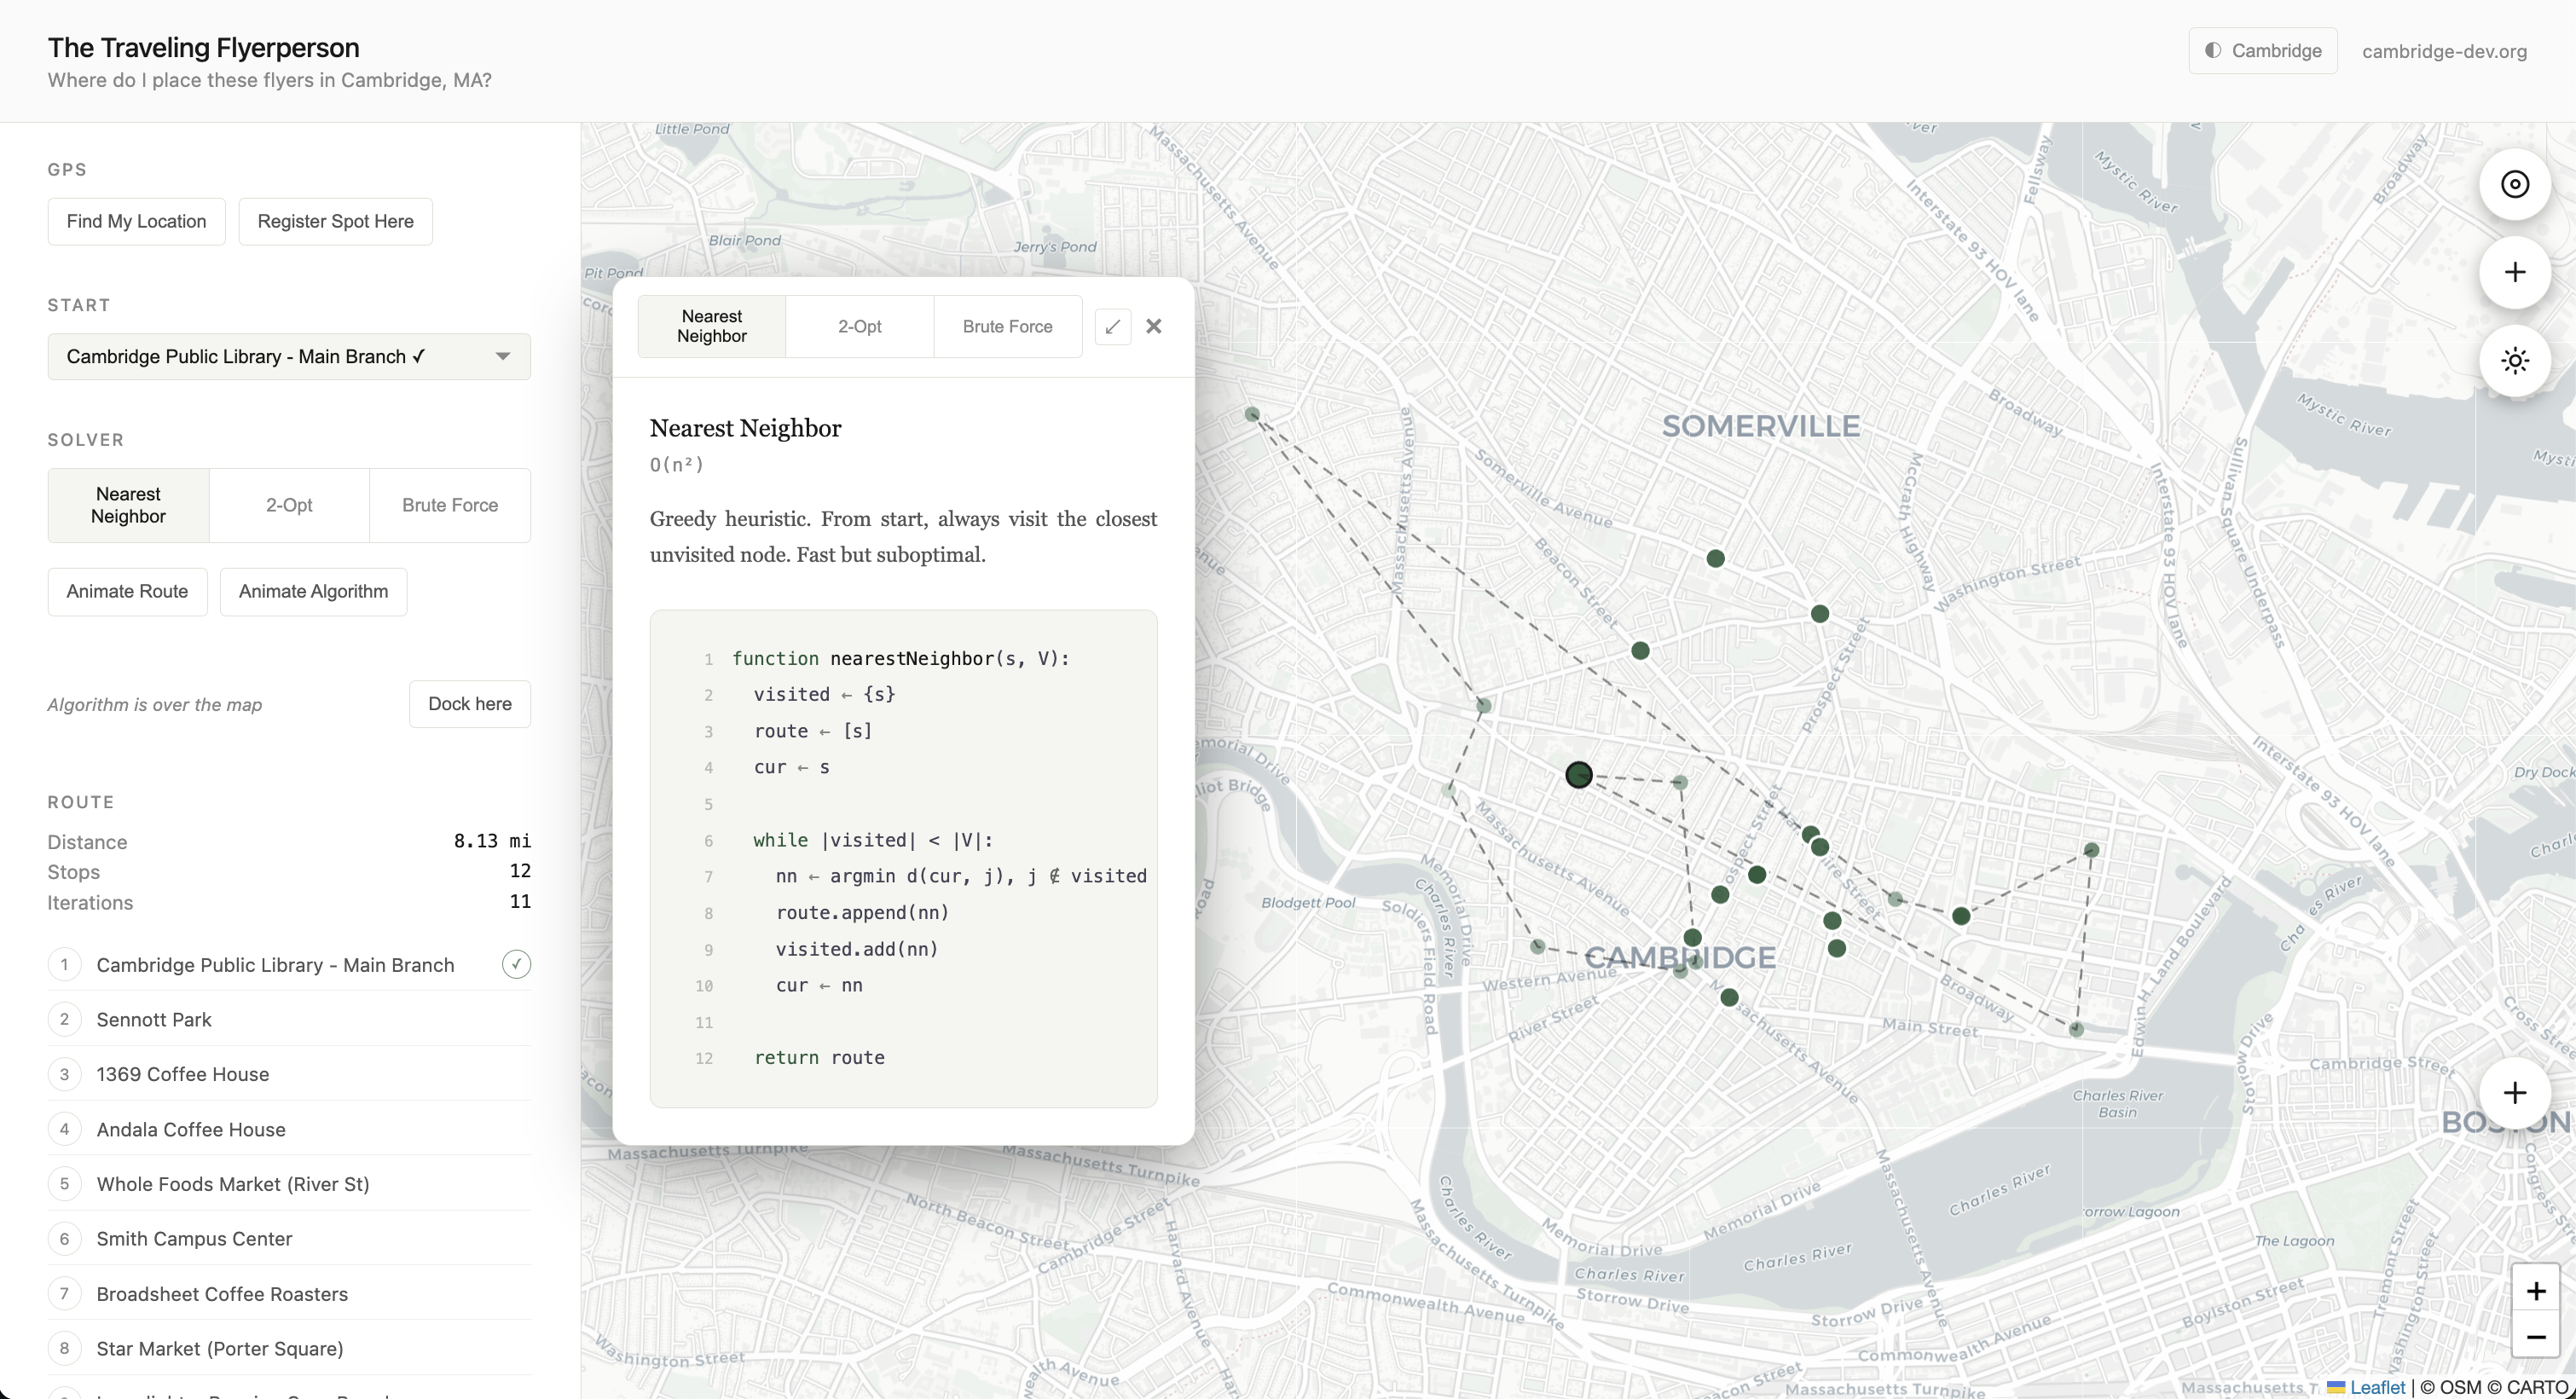
\includegraphics[width=\linewidth]{figures/app-desktop-2.png}
    \caption{The algorithm panel popped out over the map. Pseudocode is rendered with line numbers and syntax highlighting; the active line is illuminated as the route is built step by step, mirroring a debugger's stepping behavior.}
    \label{fig:desktop2}
\end{figure}

\begin{figure}[t]
    \centering
    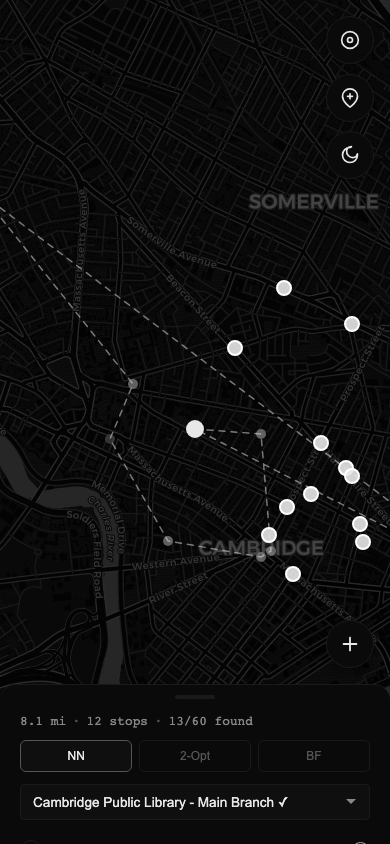
\includegraphics[width=0.55\linewidth]{figures/app-mobile.png}
    \caption{Mobile layout. Top FABs handle GPS, spot registration, and theme; bottom FABs expand into route animation, algorithm-step animation, and an algorithm-info overlay. The bottom sheet swipes between collapsed, peek, and full states.}
    \label{fig:mobile}
\end{figure}

\subsection{Routing as a Traveling Salesman Problem}

Let $V = \{v_1, \dots, v_n\}$ be a set of candidate flyer locations with coordinates $\mathbf{x}_i \in \mathbb{R}^2$ and let $D \in \mathbb{R}^{n \times n}$ be the symmetric Haversine distance matrix. A tour is a permutation $\pi$ of $\{1, \dots, n\}$ starting at a fixed origin $s$, with cost
\begin{equation}
    \mathcal{C}(\pi) = \sum_{i=1}^{n-1} D_{\pi(i), \pi(i+1)} + D_{\pi(n), \pi(1)}.
\end{equation}
We want $\pi^\star = \arg\min_\pi \mathcal{C}(\pi)$ subject to $\pi(1) = s$. The application exposes three solvers:
\begin{itemize}
    \item \textbf{Nearest Neighbor (NN)}: a greedy $O(n^2)$ heuristic.
    \item \textbf{2-Opt}: an $O(n^2 \cdot k)$ improvement heuristic seeded with NN, converging to a local minimum under segment-reversal moves.
    \item \textbf{Brute Force}: $O(n!)$ exhaustive enumeration with memoization for small $n$.
\end{itemize}
Pseudocode for each solver is rendered alongside the map (Figure~\ref{fig:desktop2}) and a step-indexed predicate marks the active region of the algorithm during animation. This pedagogical move---treating the algorithm as a first-class visual artifact, not just a function call---is the application's primary affordance for non-specialists \cite{tutorial-thompson}.

\subsection{Evidence Registry and Census}

A flyering campaign is only as credible as its receipts. Each photograph the operator takes of a placed flyer is parsed for EXIF GPS coordinates by a Node script (\texttt{scripts/extract-photo-exif.ts}) and copied into \texttt{static/evidence/} with a timestamped slug. The resulting JSON registry is bundled at build time and rendered as a separate map layer with click-through evidence cards. A simple ``Flyer Census'' panel reports observed photographs against an estimated city-wide population $\hat{N}_{\text{flyer}}$ to give the operator a calibrated sense of coverage. This is the part of the project that drives the statistical formalism in the next sections: every photograph is an observation, and every observation is intermittent.

\subsection{OpenStreetMap Covariate Layers}

The application bundles three OSM-derived layers: traffic signals ($\sim$1{,}000 nodes), bulletin board candidates ($\sim$275 amenities tagged as cafes, libraries, community centers, or bookshops), and transit points ($\sim$50 stations). These are toggleable on the map and, more importantly, serve as the empirical scaffolding for the spatial covariate vector $\mathbf{Z}(\mathbf{x})$ used in Sections~\ref{sec:point-process}--\ref{sec:bhm}.

\section{Survival Analysis under Interval Censoring}
\label{sec:survival}

Estimating how long a flyer lasts on a board is the canonical interval-censored problem. The operator does not stand watch over the bulletin board; they pass by it. For flyer $i$, the removal time $T_i$ is observed only to lie in an interval $(L_i, R_i]$ where $L_i$ is the last visit at which the flyer was intact and $R_i$ is the first visit at which it was gone or covered \cite{turnbull, robust-survival}. Naively imputing the midpoint or the right endpoint biases the survival curve in directions that depend on the local visit cadence \cite{kpke}.

\subsection{Turnbull Non-Parametric Maximum Likelihood}

Let the observed intervals be $\{(L_i, R_i]\}_{i=1}^n$. Sort and deduplicate the union $\{L_i\} \cup \{R_i\}$ into grid points $0 = t_0 < t_1 < \dots < t_m$, partitioning the timeline into disjoint intervals $I_j = (t_{j-1}, t_j]$ with probability mass $p_j$ subject to $p_j \geq 0$ and $\sum_j p_j = 1$ \cite{gte}. Define the indicator
\begin{equation}
    \alpha_{ij} = \mathbb{1}[I_j \subseteq (L_i, R_i]].
\end{equation}
The interval-censored likelihood is
\begin{equation}
    \mathcal{L}(\mathbf{p}) = \prod_{i=1}^n \sum_{j=1}^m \alpha_{ij} p_j.
\end{equation}
Direct maximization is intractable, so we use Turnbull's EM iteration: the expected event count in interval $j$ is
\begin{equation}
    \mu_j^{(k+1)} = \sum_{i=1}^n \frac{\alpha_{ij} p_j^{(k)}}{\sum_{\ell} \alpha_{i\ell} p_\ell^{(k)}},
\end{equation}
and the updated mass is $p_j^{(k+1)} = \mu_j^{(k+1)} / n$. The iteration terminates when $\max_j |p_j^{(k+1)} - p_j^{(k)}| < \epsilon$. The estimated survival is $\hat{S}(t) = \sum_{j : t_j > t} p_j$.

\subsection{Parametric AFT and Bayesian Regularization}

The Turnbull NPMLE is consistent but unstable when $n$ is small and event prevalence is low---a regime we are squarely in for any single neighborhood. We complement it with a Weibull accelerated failure time (AFT) model, $T_i \mid \mathbf{z}_i \sim \text{Weibull}(k, \lambda_i)$ with $\log \lambda_i = \mathbf{z}_i^\top \boldsymbol{\beta}$, embedded in a Bayesian framework with regularizing priors on $\boldsymbol{\beta}$ and $k$ \cite{robust-survival}. Table~\ref{tab:survival} compares the four candidate techniques on the criteria that matter operationally: censoring handling, shape recovery, small-sample robustness, and extrapolation validity.

\begin{table}[t]
    \centering
    \small
    \caption{Comparison of survival modeling techniques for flyer lifespan estimation.}
    \label{tab:survival}
    \begin{tabular}{p{2.0cm}p{1.6cm}p{1.6cm}p{1.6cm}}
        \toprule
        Technique & Censoring & Small-$n$ & Extrapolation \\
        \midrule
        Kaplan-Meier & right only & moderate & infeasible \\
        Turnbull NPMLE & arbitrary & low & poor \\
        Weibull AFT & arbitrary & high & high \\
        Bayesian piecewise exp. & arbitrary & high & excellent \\
        \bottomrule
    \end{tabular}
\end{table}

\section{Spatial Point Processes and Thinning}
\label{sec:point-process}

Let $W \subset \mathbb{R}^2$ be the bounded study region of Cambridge, and let $\mathbf{X} = \{\mathbf{x}_1, \dots, \mathbf{x}_N\} \subset W$ be the realized locations of active flyers. Under the inhomogeneous Poisson point process (IPPP) model, the count $N(B)$ of flyers in $B \subseteq W$ is Poisson with mean $\Lambda(B) = \int_B \lambda(\mathbf{x}) \, d\mathbf{x}$, where $\lambda(\mathbf{x})$ is the first-order intensity \cite{moraga, baddeley}. We model the log-intensity as a loglinear function of covariates with an additive spatial random effect:
\begin{equation}
    \log \lambda(\mathbf{x}) = \mathbf{Z}(\mathbf{x})^\top \boldsymbol{\beta} + U(\mathbf{x}),
\end{equation}
where $U \sim \text{LGCP}$ accounts for unobserved spatial autocorrelation \cite{bstpp, spatstat-poisson}. Estimation of $\boldsymbol{\beta}$ proceeds via the score equation
\begin{equation}
    \sum_{i=1}^N \mathbf{Z}(\mathbf{x}_i) - \int_W \mathbf{Z}(\mathbf{x}) \lambda(\mathbf{x}) \, d\mathbf{x} = \mathbf{0},
\end{equation}
with the integral approximated by a stratified grid of dummy quadrature points across Cambridge \cite{loh-yue}.

\subsection{Non-Stationary Thinning}

Once placed, each flyer is independently subject to removal. If the survival probability at coordinate $\mathbf{x}$ up to inspection time $t$ is $S(t \mid \mathbf{x})$, the surviving process is itself an IPPP with thinned intensity
\begin{equation}
    \lambda_t(\mathbf{x}) = \lambda_0(\mathbf{x}) \cdot S(t \mid \mathbf{x}).
\end{equation}
In Cambridge, $S(t \mid \mathbf{x})$ is highly non-stationary. Massachusetts General Laws Chapter 30A and local ordinances prohibit posting on public utility poles, lamp posts, shade trees, public buildings, and sidewalks; legitimate postings are confined to private community boards \cite{cambridge-redditB, duke-ordinances}. Within Business Improvement Districts such as Central Square, dedicated maintenance crews remove unauthorized postings on a daily cadence \cite{cambridge-redditA}. Institutional policies---most notably MIT Policy 12.6---reserve campus boards for recognized groups and exclude commercial postings outright \cite{mit-policy}. The net effect is a thinning kernel that collapses to near zero on public infrastructure and remains high on private interior boards.

\section{Multi-Armed Bandits for Sequential Allocation}
\label{sec:bandits}

Allocating a finite stack of flyers to a finite set of boards, with noisy feedback and spatial correlation, is a sequential decision problem. We model the conversion function $f : W \to \mathbb{R}$ as a draw from a Gaussian process,
\begin{equation}
    f \sim \mathcal{GP}(m(\cdot), k(\cdot, \cdot)),
\end{equation}
where $k$ is a Mat\'ern or squared-exponential kernel encoding spatial smoothness \cite{gp-bandits, gp-ucb}. After observing $\{(\mathbf{x}_t, y_t)\}_{t=1}^T$ with $y_t = f(\mathbf{x}_t) + \epsilon_t$, posterior mean $\mu_T$ and variance $\sigma_T^2$ are computed by standard GP regression formulas.

\paragraph{GP-UCB.} The standard acquisition rule is
\begin{equation}
    \mathbf{x}_{t+1} = \arg\max_{\mathbf{x} \in W} \left[ \mu_t(\mathbf{x}) + \beta_t^{1/2} \sigma_t(\mathbf{x}) \right].
\end{equation}
Theoretical bounds on $\beta_t$ are loose; randomized $\beta_t$ improves empirical performance while preserving sub-linear regret \cite{rgpucb}.

\paragraph{Contextual GP-UCB (CGP-UCB).} Conversion depends on time-varying context $\mathbf{c}_t$ (weather, academic calendars, transit disruptions). We extend $f$ to the joint space $W \times \mathcal{C}$ with composite kernel
\begin{equation}
    k_{\text{joint}}((\mathbf{x}, \mathbf{c}), (\mathbf{x}', \mathbf{c}')) = k_{\text{spatial}}(\mathbf{x}, \mathbf{x}') \cdot k_{\text{context}}(\mathbf{c}, \mathbf{c}'),
\end{equation}
allowing the agent to extrapolate across both space and time \cite{cgpucb, cgpucb-eth}.

\paragraph{HyperPrior Thompson Sampling (HP-GP-TS).} When the GP hyperparameters (length scale, signal variance) are themselves uncertain, we maintain a hyperprior over a discrete set of candidate kernel configurations $\Theta = \{\theta_1, \dots, \theta_K\}$ and at each step (i) draw $\theta \sim p_t(\theta)$, (ii) draw $\tilde{f} \sim \mathcal{GP}_\theta$, (iii) play $\mathbf{x}_{t+1} = \arg\max \tilde{f}$, and (iv) update $p_{t+1}(\theta) \propto p_t(\theta) \cdot p(y_{t+1} \mid \mathbf{x}_{t+1}, \theta)$ \cite{hpts}. This bi-level posterior accelerates learning by quickly discarding misspecified spatial-correlation models.

\section{Engagement Latency Across Amenity Types}
\label{sec:latency}

Conversion is mediated by \emph{engagement latency}: the duration and depth of attention a pedestrian allocates to a board. This varies by an order of magnitude across amenity types. Table~\ref{tab:latency} summarizes the empirical profile we use as an informative prior in Section~\ref{sec:bhm}.

\begin{table*}[t]
    \centering
    \small
    \caption{Engagement profile by amenity type (Cambridge, MA).}
    \label{tab:latency}
    \begin{tabular}{lllll}
        \toprule
        Amenity & Dwell time & Cognitive focus & Policing frequency & Conversion elasticity \\
        \midrule
        Laundromats & 30--120 min & low & low (private interior) & high \\
        Cafes & 15--60 min & low--moderate & moderate (curated) & high \\
        Libraries & 60--180 min & high (task-focused) & low (curated) & moderate \\
        Transit shelters & 5--20 min & high (situational) & high (MBTA crews) & low \\
        Utility poles (public) & seconds & high (navigation) & extreme (BID sweeps) & negligible \\
        \bottomrule
    \end{tabular}
\end{table*}

\section{Bayesian Hierarchical Predictive Framework}
\label{sec:bhm}

We synthesize the components above into a three-level hierarchical model that predicts expected conversion at each candidate location $i \in \{1, \dots, n\}$ over an evaluation horizon $\Delta t$.

\paragraph{Level 1 (Observation).} Observed conversions follow a Poisson likelihood,
\begin{align}
    Y_i &\sim \text{Poisson}(\mu_i), \\
    \mu_i &= F_i \cdot \rho_i \cdot S_i(\Delta t) \cdot \gamma_i,
\end{align}
where $F_i$ is the number of flyers placed, $\rho_i$ is the pedestrian traffic density at location $i$ (estimated by KDE over MBTA boarding volumes), $S_i(\Delta t)$ is the survival probability, and $\gamma_i$ is the latent conversion probability per exposure.

\paragraph{Level 2 (Latent parameters).} The conversion logit and survival parameters are
\begin{align}
    \mathrm{logit}(\gamma_i) &= \beta_0 + \beta_1 \log d_i + \beta_2 r_i + \boldsymbol{\beta}_a^\top \mathbf{a}_i + u_i, \\
    \log h_i &= \alpha_0 + \alpha_1 r_i + \boldsymbol{\alpha}_a^\top \mathbf{a}_i + v_i, \\
    S_i(t) &= \exp\!\left[-\left(t / \exp(\alpha_0 + \alpha_1 r_i + \boldsymbol{\alpha}_a^\top \mathbf{a}_i)\right)^\kappa\right],
\end{align}
where $d_i$ is dwell time, $r_i$ is the regulatory risk index, $\mathbf{a}_i$ is a one-hot amenity vector, and $(u_i, v_i)$ are spatial random effects drawn jointly from a Gaussian process with Mat\'ern kernel
\begin{equation}
    k(\mathbf{x}, \mathbf{x}') = \sigma^2 \cdot \frac{2^{1-\nu}}{\Gamma(\nu)} \left(\frac{\sqrt{2\nu} \, \|\mathbf{x} - \mathbf{x}'\|}{\ell}\right)^\nu K_\nu\!\left(\frac{\sqrt{2\nu} \, \|\mathbf{x} - \mathbf{x}'\|}{\ell}\right).
\end{equation}

\paragraph{Level 3 (Priors).} We place weakly informative priors,
\begin{align}
    \boldsymbol{\beta}, \boldsymbol{\alpha} &\sim \mathcal{N}(\mathbf{0}, 10 \mathbf{I}), \\
    \kappa &\sim \text{LogNormal}(0, 1), \\
    \sigma^2 &\sim \text{InvGamma}(2, 1), \\
    \ell &\sim \text{InvGamma}(2, 1).
\end{align}

By sharing strength across the hierarchy, the model produces a posterior on $\gamma_i$ for previously unvisited boards by leveraging covariate-similar boards elsewhere in the city---exactly what the GP bandit needs to seed itself.

\subsection{Reference Implementation}

A self-contained Python prototype implementing this model is included with the project. The class \texttt{BayesianSpatialFlyerOptimizer} ingests \texttt{locations.json} and \texttt{transit.json}, computes a KDE-based pedestrian density surface, applies a Turnbull-adjusted Weibull survival per amenity, and runs a Metropolis-within-Gibbs MCMC sampler over $\boldsymbol{\beta}$ with weakly informative priors. The output is a structured posterior heatmap of expected conversions per ten flyers placed, by location.

\begin{algorithm}[t]
\caption{Metropolis-within-Gibbs for $\boldsymbol{\beta}$}
\label{alg:mh}
\begin{algorithmic}[1]
\State Initialize $\boldsymbol{\beta}^{(0)} = \mathbf{0}$, proposal covariance $\Sigma_q$
\For{$s = 1, \dots, T$}
    \State Propose $\boldsymbol{\beta}^\star \sim \mathcal{N}(\boldsymbol{\beta}^{(s-1)}, \Sigma_q)$
    \State Compute log-posterior $\log p(\boldsymbol{\beta}^\star \mid \mathbf{Y})$
    \State Compute acceptance ratio $r = \log p(\boldsymbol{\beta}^\star) - \log p(\boldsymbol{\beta}^{(s-1)})$
    \If{$r > \log u$, $u \sim \text{Uniform}(0,1)$}
        \State $\boldsymbol{\beta}^{(s)} \gets \boldsymbol{\beta}^\star$
    \Else
        \State $\boldsymbol{\beta}^{(s)} \gets \boldsymbol{\beta}^{(s-1)}$
    \EndIf
\EndFor
\State Discard burn-in, return posterior mean and standard deviation.
\end{algorithmic}
\end{algorithm}

\section{Synthesis and Recommendations}
\label{sec:synthesis}

The model and the application converge on three operational guidelines.

\paragraph{Exploit the laundromat-cafe capture effect.} Raw foot traffic is misleading. Transit shelters generate orders of magnitude more raw exposures than community laundromats, but yield lower net conversions due to truncated dwell times and high cognitive load \cite{transit-volumes}. Concentrating placement on private interior boards in laundromats, cafes, and student co-ops maximizes engagement latency and, given low policing frequency, extends Weibull lifespan by a factor of fifty or more.

\paragraph{Mitigate legal and institutional cleaning filters.} Public utility poles and BID-policed commercial districts are essentially zero-survival zones \cite{cambridge-redditA, cambridge-redditB}. The MIT campus is a localized exclusion zone under Policy 12.6 \cite{mit-policy}. The model's thinning component flags these regions automatically.

\paragraph{Deploy spatial bandits for territory expansion.} Once a base set of high-performing boards is established, GP-UCB or HP-GP-TS over the bulletin-board candidate set from OpenStreetMap allows the operator to systematically evaluate new locations while preserving sub-linear regret. The application's evidence registry provides exactly the noisy feedback signal $y_t$ the bandit consumes.

\section{Discussion}
\label{sec:discussion}

\emph{The Traveling Flyerperson} is, materially, a small project. The deployed app fits in a single SvelteKit route. The mathematical framework is assembled from well-understood components: Turnbull's NPMLE, Poisson point processes, GP bandits, and a hierarchical Bayesian model with MCMC. None of these are novel in isolation. What we hope is novel is the framing: a civic task that a small group of people can actually do, taken seriously enough to produce a defensible end-to-end pipeline from photograph to point process.

The project is also a deliberate exercise in scope. We resist the temptation to inflate flyering into a general theory of urban media, or to claim the BHM is calibrated against ground-truth conversions we have not yet collected. The honest status, at the time of writing, is: 13 flyers placed, 13 photographs registered, an estimated population of 60 in circulation, a working route optimizer, and a documented predictive framework awaiting more observations \cite{cambridge-dev-org}.

That last clause is the point. The application's evidence registry generates exactly the data the BHM needs. Every photograph collected on a bike ride is an interval-censored observation with covariates. Over time, the empirical posterior will sharpen, the bandit will explore beyond the seed set, and the city itself becomes the experiment. The civic and the computational here are not metaphors for each other; they are the same activity.

\section{Conclusion}

We presented a deployed, mobile-first TSP visualization for flyer routing in Cambridge, MA, and a unified Bayesian hierarchical framework that reframes the placement problem as a predictive estimation task combining survival analysis, spatial point processes, and contextual bandits. The artifact is small, the framework is defensible, and the data pipeline is closed. If the project has a thesis, it is that community-scale computing benefits from being held to research-grade rigor, and research-grade rigor benefits from being grounded in a task someone can actually do on a Tuesday afternoon in Cambridge.

\section*{Acknowledgments}

This work was developed under the umbrella of \texttt{cambridge-dev}. We thank the public bulletin boards of Cambridge, MA, and the operators of the laundromats, cafes, and libraries that host them.

\begin{thebibliography}{99}

\bibitem{cambridge-dev-org}
cambridge-dev. \url{https://www.cambridge-dev.org/}, accessed May 2026.

\bibitem{cambridge-redditA}
r/CambridgeMA. ``Legality of Flyer-ing?'' Reddit thread. \url{https://www.reddit.com/r/CambridgeMA/comments/1qduyek/legality_of_flyering/}, accessed May 2026.

\bibitem{cambridge-redditB}
r/CambridgeMA. ``Can you get in trouble for posting flyers on community boards in Boston?'' Reddit thread. \url{https://www.reddit.com/r/CambridgeMA/comments/1t9ondy/}, accessed May 2026.

\bibitem{mit-policy}
Massachusetts Institute of Technology. \emph{Policy 12.6: Bulletin Boards, Postering, and Display Spaces.} \url{https://policies.mit.edu/policies-procedures/120-relations-public-use-mit-name-and-facilities-use/126-bulletin-boards}, accessed May 2026.

\bibitem{duke-ordinances}
Duke Law School First Amendment Clinic. \emph{Municipal Ordinances Spreadsheet.} April 2025.

\bibitem{turnbull}
B. W. Turnbull. ``The empirical distribution function with arbitrarily grouped, censored, and truncated data.'' \emph{J. R. Stat. Soc. B}, 38(3):290--295, 1976.

\bibitem{robust-survival}
Authors. ``Robust Survival Estimation under Interval Censoring: EM and Bayesian AFT Assessment.'' \emph{arXiv:2509.02634}, 2025.

\bibitem{kpke}
Authors. ``Evaluation of a Non-Parametric Penalized Kaplan-Meier Estimator Under Interval-Censored Survival Data.'' \emph{Symmetry}, 18(3):519, 2026.

\bibitem{gte}
\texttt{gte}: Generalized Turnbull's Estimator. R package documentation, RDocumentation, 2024.

\bibitem{moraga}
P. Moraga. \emph{Spatial Statistics for Data Science: Theory and Practice with R.} Chapter 19, ``Spatial point processes and simulation.''

\bibitem{baddeley}
A. Baddeley. \emph{Spatial Point Processes and their Applications.} Lecture notes, Virginia Tech.

\bibitem{bstpp}
Authors. ``BSTPP: a Python package for Bayesian spatiotemporal point processes.'' PMC12490397, 2025.

\bibitem{spatstat-poisson}
A. Baddeley, R. Turner, E. Rubak. \emph{Spatial Point Patterns: Methodology and Applications with R.} Chapter 9, Poisson Models.

\bibitem{loh-yue}
J.-M. Loh, S. Yue. ``Variable Selection for Inhomogeneous Spatial Point Process Models.'' \emph{Canadian Journal of Statistics}, 2015.

\bibitem{tutorial-thompson}
D. Russo, B. Van Roy, A. Kazerouni, I. Osband, Z. Wen. \emph{A Tutorial on Thompson Sampling.} Stanford University, 2018.

\bibitem{gp-bandits}
E. Mathieu. \emph{Gaussian Process Bandits.} Course report.

\bibitem{gp-ucb}
N. Srinivas, A. Krause, S. Kakade, M. Seeger. ``Gaussian Process Optimization in the Bandit Setting: No Regret and Experimental Design.'' \emph{ICML}, 2010.

\bibitem{rgpucb}
Authors. ``Randomised Gaussian Process Upper Confidence Bound for Bayesian Optimisation.'' \emph{IJCAI}, 2020.

\bibitem{cgpucb}
A. Krause, C. Ong. ``Contextual Gaussian Process Bandit Optimization.'' \emph{NeurIPS}, 2011.

\bibitem{cgpucb-eth}
Learning \& Adaptive Systems Group, ETH Zurich. ``Contextual Gaussian Process Bandit Optimization.''

\bibitem{hpts}
Authors. ``Efficient Prior Selection in Gaussian Process Bandits with Thompson Sampling.'' \emph{arXiv:2502.01226}, 2025.

\bibitem{transit-volumes}
NYC Department of Transportation. \emph{Downtown Brooklyn Surface Transit Circulation Study Final Report.}

\end{thebibliography}

\end{document}
